% !TeX root = main.tex
\documentclass[conference]{IEEEtran}
\usepackage{cite}
\usepackage{amsmath,amssymb,amsfonts}
\usepackage{algorithmic}
\usepackage{graphicx}
\usepackage{textcomp}
\usepackage{xcolor}
\def\BibTeX{{\rm B\kern-.05em{\sc i\kern-.025em b}\kern-.08em
    T\kern-.1667em\lower.7ex\hbox{E}\kern-.125emX}}
\begin{document}
\title{Assignment 1\\INFOMDPLR}
\author{\IEEEauthorblockN{Cas Denteneer}
	\IEEEauthorblockA{
		\textit{0925519}\\
		\textit{c.denteneer1@students.uu.nl}}
	\and
	\IEEEauthorblockN{Jeroen Lombaers}
	\IEEEauthorblockA{
		\textit{6867553} \\
		\textit{j.j.h.lombaers@students.uu.nl}}
	\and
	\IEEEauthorblockN{Lara Timmers}
	\IEEEauthorblockA{
		\textit{7098308} \\
		\textit{l.e.timmers@students.uu.nl}}
	\and
	\IEEEauthorblockN{Laurens van Ballegooijen}
	\IEEEauthorblockA{
		\textit{9869980}\\
		\textit{l.e.f.vanballegooijen@students.uu.nl}}
}
\date{\today}
\maketitle

\section{Abstract}
The value of a laser measurement is predicted using Recurrent Neural Networks (RNNs).
A dataset of a laser measurement is scaled (using Sklearn) and used to train two types of RNNs.
These are the PyTorch implementations of Long Short-Term Memory (LSTM) and Gated Recurrent Unit (GRU).
Their performance is then measured using Mean Absolute Error (MAE) and Mean Squared Error (MSE).
The best performing model was GRU with MSE as the loss function, which yields an MAE of 49.7 and an MSE of 4103.
The model was able to capture the initial nature of the data but struggled to adapt to a subsequent change in the signal's behavior.
We find that GRU and LSTM are capable of learning patterns in sequential data, though they may struggle with variation.

\section{Introduction}
The task is to predict the value of a laser measurement using a neural network.
First, a real-life dataset of a laser measurement is given.
This data needs to be scaled before training.
We then need to train a neural network model to predict one step ahead of data point.
After training, the data is scaled back so that the model's predictions can be compared with the real measurements.

% Recurrent neural networks (RNNs) are a type of neural networks that are specialized for processing sequential data \cite{Goodfellow2016}.

\section{Methodology}
The laser measurement is a type of sequential data. To predict further values we apply two different Recurrent Neural Networks (RNNs), which process sequential data by retaining information from previous steps. The models we choose are discussed further in the corresponding subsection. We preprocess the data by scaling with the \texttt{MinMaxscaler()} from Sklearn, which scales the data linearly between values 0 and 1. We optimize the models using grid search to obtain the best configuration of hyperparameters. We measure their performance with the Mean Absolute Error (MAE) and Mean Squared Error (MSE), given by
\begin{align}
	\mathrm{MAE} & = \frac{1}{n} \sum_{i=1}^{n} | y_i - \hat{y}_i |, \,\,\, \mathrm{MSE} & = \frac{1}{n} \sum_{i=1}^{n} (y_i - \hat{y}_i)^2,
\end{align}
where $y_i$ is the real value and $\hat{y}_i$ the value predicted by the model. After obtaining the test data we apply the best model with the best hyperparameter configuration we obtained during the training phase and report its performance.

\subsection{Models}
The models we used are Long Short-Term Memory (LSTM) and Gated Recurrent Unit (GRU) RNN's from PyTorch. RNN's can predict sequential data by looking back to previous steps, making it suitable for our task. We chose to use LSTM and GRU because they are the most effective sequence models used in practical applications \cite{Goodfellow2016}.

LSTM's work by allowing information to persist from one inference to the next \cite{Noble2025}. An LSTM looks at an input $X_t$ and outputs a value $H_t$. Through loops, information from each input-output cycle gets passed on to the next step in the network. The strength of the LSTM over other traditional RNN's is a type of storage it has that is called the memory cell. With this cell, the LSTM maintains a persistent "cell state" to store information long-term across multiple time steps. This enables it to continuously pass information from previous input-output cycles while simultaneously using gates to selectively add, remove or update information \cite{Noble2025}.

The memory cell consists of three gates: the input, output, and forget gate.
\begin{equation}
	\begin{aligned}
		i_t = \sigma(W_i h_{t-1},x_t+b_i) \\
		o_t = \sigma(W_o h_{t-1},x_t+b_o) \\
		f_t = \sigma(W_f h_{t-1},x_t+b_f)
	\end{aligned}
\end{equation}

As the names suggest, each gate is responsible for moving information to subsequent gates or hidden states. The forget gate acts first, screening what information from the previous time step to retain or forget. The input gate takes information in and determines what information to pass to memory, and finally the output gate decides what part of the internal state gets passed on to the next hidden state.

Similar to the LSTM architecture, the GRU architecture is designed to model sequential time-series data. Both architectures allow to iteratively select what information to remember and discard, only keeping the most relevant data for accurate predictions. Compared to LSTM's, the GRU architecture is much simpler. In the LSTM, the memory cell is a separate component from the hidden state, and consists of the input, output, and forget gate. In GRU, the memory cell is replaced with a "candidate activation gate" which consists of only two gates: the reset gate, and the update gate \cite{Nama2023}. The candidate activation vector combines information from both the input and the previous hidden state and then uses the vector to update the hidden state for the next step. The reset gate and the update gate determine what information from the previous hidden state to forget and what portion of the candidate activation function to add to the new hidden state.

\begin{equation}
	\begin{aligned}r_t &= \sigma\left(\mathbf{W}_r \cdot [\mathbf{h}_{t-1}, \mathbf{x}_t]\right)\\z_t &= \sigma\left(\mathbf{W}_z \cdot [\mathbf{h}_{t-1}, \mathbf{x}_t]\right)\end{aligned}
\end{equation}

In both equations above, the sigmoid function is applied to the dot product of weight matrices $W_r$ and $W_z$ and the current input and previous hidden state to produce outputs for the reset and update gate respectively.

To correspond to the measures we use to map the performance of the models, we use the loss function \texttt{MSELoss()} from PyTorch.

As an optimizer we use Adam, which is an adaptive learning rate optimization method introduced by \cite{kingma2014adam}. Adam incorporates momentum as an estimate of the first order moment of the gradient, and it applies bias correction in response to the fact that the moments are initialized at the origin.

\section{Results}

Best number of past time steps to consider (answer to question B)

Based on our experimentation prior to applying our best models on the test data, we have found the optimal combination of model and hyperparameters, as shown in the table below.

\begin{table}[htpb]
	\centering
	\caption{Best Results per Model and Loss Function Combination}
	\label{table:model_comparison}
	\resizebox{\columnwidth}{!}{%
		\begin{tabular}{llcccc}
			\hline
			\textbf{Model} & \textbf{Loss Function} & \textbf{Interval} & \textbf{Hidden Size} & \textbf{Learning Rate} & \textbf{Validation Loss} \\ \hline
			GRU            & MSE                    & 50                & 16                   & 0.050                  & 0.\textbf{000591}        \\
			LSTM           & MSE                    & 20                & 16                   & 0.050                  & 0.000844                 \\
			LSTM           & MAE                    & 50                & 32                   & 0.10                   & 0.018310                 \\
			GRU            & MAE                    & 5                 & 16                   & 0.10                   & 0.019853                 \\ \hline
		\end{tabular}%
	}
	\label{table:model_comparison}
\end{table}

As shown in Table \ref{table:model_comparison}, the best model based on our tuning, is the GRU model with Mean Squared Error (MSE) as the loss function. In combination with an interval of 50, hidden size 16, and a learning rate of 0.05, the validation loss comes out to an effective 0.000591. Combining a high look-back interval with a smaller hidden size of 16 allowed the model to still oscillate enough for accurate predictions, without shooting too far beyond the actual data points. With a validation loss almost 50\% lower than the next best model combination solidifies this model combination as the most effective for testing.

\subsection{Testing}
We compare the results from the best configuration of hyperparameters of the best model to the test data. The model we found was GRU with MSE Loss, and the evaluation of its prediction compared to the actual test data yields an MAE of 49.7 and a MSE of 4103.
In figure \ref{fig:realvspred} we see that the real data oscillation suddenly drops in amplitude, which explain the high MSE and MAE values. MSE is more sensitive to outliers, which explains why the MSE value is much higher then the MAE.
The model also does not seem to adjust to a change in the period of the oscillation in the laser movement, which is visible at the first 70 steps.

\begin{figure}
	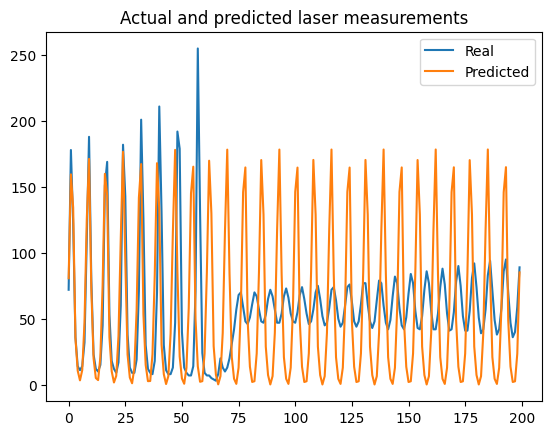
\includegraphics[width=\linewidth]{testvspred.png}
	\caption{Actual laser measurement and predicted laser trajectory by GRU RNN with MSELoss and hyperparameters values \textit{interval} 30, \textit{hidden\_size}: 64, and \textit{learning rate}: 0.01.}
	\label{fig:realvspred}
\end{figure}

\section{Conclusion}
In this assignment, we used recurrent neural networks to predict future values of a laser measurement time series.
After scaling the data, LSTM and GRU models were trained and optimized through a grid search over several hyperparameters.
The GRU model with MSE loss achieved the best validation performance with an interval of 50 past time steps, hidden size 16, and learning rate 0.05.

When applied to the test data, the model was able to capture the general oscillatory behavior of the signal but struggled with changes in amplitude and period.
This resulted in relatively high MAE and MSE values, especially MSE because it is sensitive to larger prediction errors.
In conclusion, the results show that LSTM and GRU can learn temporal patterns in the data, but struggle with variation, resulting in a prediction for our test case that is significantly different.

\bibliographystyle{IEEEtran}
\bibliography{bibliography}

\end{document}
